\section{随机游走：从局部步进到整体尺度}
\label{sec:06-Random-Processes/04-Applications/01}

十行代码就能跑出来：从 \(0\) 出发，每步以相等的概率加一或减一，走满一万步，记下终点；重复一千次。这一千个终点的绝对值，中位数落在 \(67\) 附近，超过 \(300\) 的通常只有两三次。

脚下的总路程是一万，净位移只有几十。

如果你原本的预期是``走得越久离原点越远''，这个数并不反驳它——位移确实在长大。落空的是长大的速度。多数人心里那个隐含的比例是线性的：步数翻四倍，距离也该翻四倍。实际只翻两倍。步数与位移之间隔着一个平方根，而这个平方根不是随机游走的特产，它是一切由独立小扰动累积起来的量所共有的标度。

\subsection{可加的是方差，不是标准差}

单步增量 \(Z_k\) 取 \(\pm1\)，均值为零，平方恒等于一，所以 \(\Var(Z_k)=1\)。位置是它们的和，\(S_n=Z_1+\cdots+Z_n\)。期望的线性性直接给出 \(\E[S_n]=0\)；独立性让所有交叉项 \(\Cov(Z_j,Z_k)\) 归零，于是方差逐项相加：

\[
\begin{aligned}
\Var(S_n)&=\sum_{j,k}\Cov(Z_j,Z_k)=\sum_{k=1}^{n}\Var(Z_k)=n,\\
\sqrt{\Var(S_n)}&=\sqrt n.
\end{aligned}
\]

推导两行，结论却常被记反。相加的是方差；标准差作为它的平方根，只能按 \(\sqrt n\) 长。一万步给出 \(\sqrt{10000}=100\)，而模拟里的中位数是 \(67\)——因为标准正态取绝对值后的中位数约为 \(0.67\)，两个数是对得上的。

换成一般的单步分布，只要各步独立、均值为零、方差为 \(\sigma^2\) 有限，同样的两行给出 \(\sqrt{\Var(S_n)}=\sigma\sqrt n\)。硬币的细节被吸收进 \(\sigma\)，标度不变。

\begin{center}
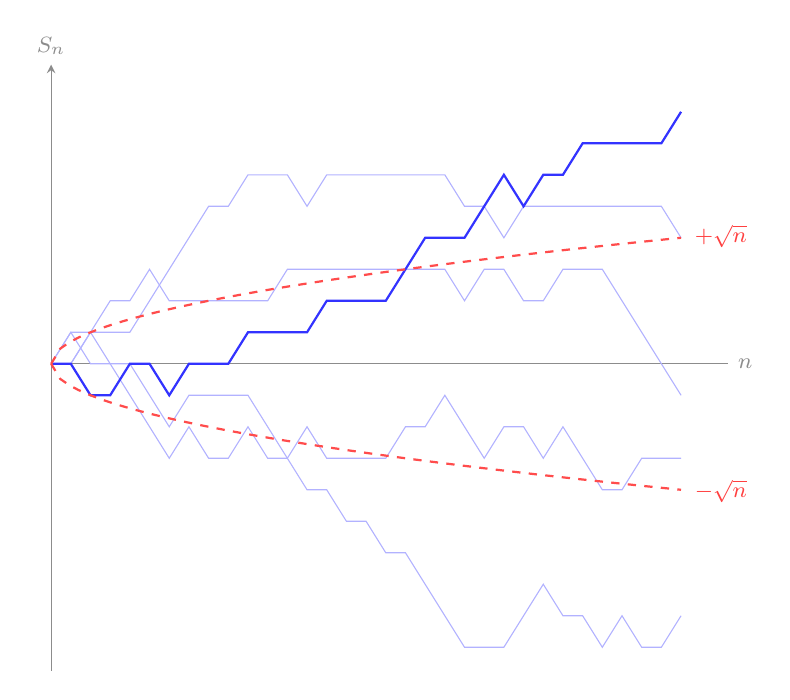
\begin{tikzpicture}[x=1cm,y=1cm,font=\small,>=stealth]
  \draw[black!45] (0,0) -- (8.6,0) node[right,font=\footnotesize] {\(n\)};
  \draw[->,black!45] (0,-3.9) -- (0,3.8) node[above,font=\footnotesize] {\(S_n\)};
  \draw[blue!30] (0.00,0.00) -- (0.25,0.00) -- (0.50,0.40) -- (0.75,0.00) -- (1.00,0.00) -- (1.25,-0.40) -- (1.50,-0.80) -- (1.75,-0.40) -- (2.00,-0.40) -- (2.25,-0.40) -- (2.50,-0.40) -- (2.75,-0.80) -- (3.00,-1.20) -- (3.25,-1.60) -- (3.50,-1.60) -- (3.75,-2.00) -- (4.00,-2.00) -- (4.25,-2.40) -- (4.50,-2.40) -- (4.75,-2.80) -- (5.00,-3.20) -- (5.25,-3.60) -- (5.50,-3.60) -- (5.75,-3.60) -- (6.00,-3.20) -- (6.25,-2.80) -- (6.50,-3.20) -- (6.75,-3.20) -- (7.00,-3.60) -- (7.25,-3.20) -- (7.50,-3.60) -- (7.75,-3.60) -- (8.00,-3.20);
  \draw[blue!30] (0.00,0.00) -- (0.25,0.40) -- (0.50,0.00) -- (0.75,0.00) -- (1.00,-0.40) -- (1.25,-0.80) -- (1.50,-1.20) -- (1.75,-0.80) -- (2.00,-1.20) -- (2.25,-1.20) -- (2.50,-0.80) -- (2.75,-1.20) -- (3.00,-1.20) -- (3.25,-0.80) -- (3.50,-1.20) -- (3.75,-1.20) -- (4.00,-1.20) -- (4.25,-1.20) -- (4.50,-0.80) -- (4.75,-0.80) -- (5.00,-0.40) -- (5.25,-0.80) -- (5.50,-1.20) -- (5.75,-0.80) -- (6.00,-0.80) -- (6.25,-1.20) -- (6.50,-0.80) -- (6.75,-1.20) -- (7.00,-1.60) -- (7.25,-1.60) -- (7.50,-1.20) -- (7.75,-1.20) -- (8.00,-1.20);
  \draw[blue!30] (0.00,0.00) -- (0.25,0.40) -- (0.50,0.40) -- (0.75,0.80) -- (1.00,0.80) -- (1.25,1.20) -- (1.50,0.80) -- (1.75,0.80) -- (2.00,0.80) -- (2.25,0.80) -- (2.50,0.80) -- (2.75,0.80) -- (3.00,1.20) -- (3.25,1.20) -- (3.50,1.20) -- (3.75,1.20) -- (4.00,1.20) -- (4.25,1.20) -- (4.50,1.20) -- (4.75,1.20) -- (5.00,1.20) -- (5.25,0.80) -- (5.50,1.20) -- (5.75,1.20) -- (6.00,0.80) -- (6.25,0.80) -- (6.50,1.20) -- (6.75,1.20) -- (7.00,1.20) -- (7.25,0.80) -- (7.50,0.40) -- (7.75,0.00) -- (8.00,-0.40);
  \draw[blue!30] (0.00,0.00) -- (0.25,0.00) -- (0.50,0.40) -- (0.75,0.40) -- (1.00,0.40) -- (1.25,0.80) -- (1.50,1.20) -- (1.75,1.60) -- (2.00,2.00) -- (2.25,2.00) -- (2.50,2.40) -- (2.75,2.40) -- (3.00,2.40) -- (3.25,2.00) -- (3.50,2.40) -- (3.75,2.40) -- (4.00,2.40) -- (4.25,2.40) -- (4.50,2.40) -- (4.75,2.40) -- (5.00,2.40) -- (5.25,2.00) -- (5.50,2.00) -- (5.75,1.60) -- (6.00,2.00) -- (6.25,2.00) -- (6.50,2.00) -- (6.75,2.00) -- (7.00,2.00) -- (7.25,2.00) -- (7.50,2.00) -- (7.75,2.00) -- (8.00,1.60);
  \draw[blue!80,thick] (0.00,0.00) -- (0.25,0.00) -- (0.50,-0.40) -- (0.75,-0.40) -- (1.00,0.00) -- (1.25,0.00) -- (1.50,-0.40) -- (1.75,0.00) -- (2.00,0.00) -- (2.25,0.00) -- (2.50,0.40) -- (2.75,0.40) -- (3.00,0.40) -- (3.25,0.40) -- (3.50,0.80) -- (3.75,0.80) -- (4.00,0.80) -- (4.25,0.80) -- (4.50,1.20) -- (4.75,1.60) -- (5.00,1.60) -- (5.25,1.60) -- (5.50,2.00) -- (5.75,2.40) -- (6.00,2.00) -- (6.25,2.40) -- (6.50,2.40) -- (6.75,2.80) -- (7.00,2.80) -- (7.25,2.80) -- (7.50,2.80) -- (7.75,2.80) -- (8.00,3.20);
  \draw[red!70,thick,dashed] plot[domain=0:8,samples=70] (\x,{0.5657*sqrt(\x)});
  \draw[red!70,thick,dashed] plot[domain=0:8,samples=70] (\x,{-0.5657*sqrt(\x)});
  \node[right,font=\footnotesize,red!75] at (8.05,1.62) {\(+\sqrt n\)};
  \node[right,font=\footnotesize,red!75] at (8.05,-1.62) {\(-\sqrt n\)};
\end{tikzpicture}

\emph{五条独立的样本轨道，各走 \(64\) 步。红色虚线是 \(\pm\sqrt n\)。它不是任何一条轨道的上界，而是典型偏离的量级：轨道在这条曲线的一两倍范围内游荡，越界一阵又被拉回。曲线越往右越平：再走一段，位移只按平方根往上挪。}
\end{center}

这条包络后面还会回来两次：一次用来解释高维格点上为什么回不了家，一次用来解释把步长缩小到极限时该按什么比例缩。

\subsection{漂移和噪声有一个交叉点}

硬币若不公平，\(p\neq 1/2\)，情况分成两截。均值以 \(\mu=p-q\) 的速率线性漂移，\(\E[S_n]=\mu n\)；波动仍然是 \(\sigma\sqrt n\)，其中 \(\sigma=2\sqrt{pq}\)。一个按 \(n\) 长，一个按 \(\sqrt n\) 长，它们必然交叉，交叉点在

\[
n^\ast=\Big(\frac{\sigma}{\mu}\Big)^{2}.
\]

\begin{center}
\begin{tikzpicture}[x=1cm,y=1cm,font=\small,>=stealth]
  \draw[->,black!50] (0,0) -- (8.7,0) node[right,font=\footnotesize] {\(n\)};
  \draw[->,black!50] (0,0) -- (0,2.95) node[above,font=\footnotesize] {偏离量级};
  \draw[blue!75,thick] (0,0) -- (8,2.5);
  \draw[red!70,thick] plot[domain=0:8,samples=70] (\x,{0.625*sqrt(\x)});
  \draw[black!35,dashed] (4,0) -- (4,1.25);
  \fill[black!75] (4,1.25) circle (1.8pt);
  \node[right,font=\footnotesize,blue!75] at (8.05,2.5) {漂移 \(\mu n\)};
  \node[right,font=\footnotesize,red!75] at (8.05,1.78) {噪声 \(\sigma\sqrt n\)};
  \node[below,font=\footnotesize] at (4,-0.06) {\(n^\ast=(\sigma/\mu)^2\)};
  \node[below,font=\footnotesize,black!70,align=center] at (1.7,-0.75) {左侧：噪声压过趋势，\\一次实现看不出方向};
  \node[below,font=\footnotesize,black!70,align=center] at (6.6,-0.75) {右侧：趋势压过噪声，\\方向稳定可读};
\end{tikzpicture}

\emph{两条曲线在 \(n^\ast\) 处交叉。交叉点左边，位移的符号基本由运气决定；右边，符号几乎总是跟着 \(\mu\) 走。所有``要收集多少数据才能看出这个效应''的问题，答案的骨架都是这个 \((\sigma/\mu)^2\)。}
\end{center}

每步只偏 \(0.02\)，\(\sigma\approx1\)，交叉点就在两千五百步之后。在此之前你看到的几乎全是噪声，此后趋势才稳定地露出来。这个数在不同场景里换着名字出现。做 A/B 实验时它是样本量公式的核心：效应量与噪声之比的平方倒数决定你需要多少观测。做小批量训练时它解释了为什么随机梯度还能收敛——\(n\) 步之后，真实梯度的贡献按 \(n\) 累积，噪声的贡献只按 \(\sqrt n\) 累积，信噪比按 \(\sqrt n\) 变好；同时它也解释了为什么接近最优点后损失会停在一个平台上，那时 \(\mu\) 本身趋于零，交叉点被推到无穷远，剩下的全是噪声（\hyperref[sec:09-Convex-Optimization/08-Nonconvex-and-Stochastic-Optimization/04]{``SGD 在期望中下降但噪声会留下平台''}把这件事写成了收敛速率）。扩散模型的前向加噪也是同一个标度：独立小噪声累加 \(t\) 步，扰动幅度按 \(\sqrt t\) 增长，噪声调度表里那些平方根不是装饰。

\subsection{大尺度上只剩一个钟形}

标度说的是宽度，形状还需要一句。由中心极限定理，只要 \(0<p<1\)，

\[
\frac{S_n-\mu n}{\sigma\sqrt n}\xrightarrow{d}\mathcal N(0,1).
\]

不管最初那枚硬币偏成什么样，标准化之后的位置分布都逼近同一条曲线。离散的加一减一在大尺度上被磨掉，留下钟形（\hyperref[sec:05-Probability/08-Limit-Theorems/03]{``中心极限定理与 Gaussian 近似''}给出了条件与误差）。

近似之外，精确分布也写得出来：若 \(n\) 步中向右 \(K\) 次，则 \(S_n=2K-n\)，于是 \(S_n\) 的分布就是 Binomial 分布的平移拉伸。这里有个容易被当成技术细节的现象——\(S_n=s\) 只在 \(s\) 与 \(n\) 同奇偶时才可能。从零出发，偶数步只能落在偶数位置。这正是上一单元所说的周期 \(2\)：所谓周期，说到底就是对可达位置的奇偶约束（见\hyperref[sec:06-Random-Processes/03-Markov-Chains/02]{``可达、通信类与周期性''}）。奇偶性并不影响 \(\sqrt n\) 标度，但它会让逐点的收敛看起来忽高忽低，做数值检查时值得知道。

\subsection{加两堵墙，扩散就变成击中问题}

在 \(0\) 与 \(N\) 处放上吸收壁，游走碰到任一端即停。公平游走从 \(i\) 出发，先到 \(N\) 的概率是 \(i/N\)，平均吸收时间是 \(i(N-i)\)。两个结论在\hyperref[sec:06-Random-Processes/03-Markov-Chains/05]{``首步分析、击中时间与吸收链''}里由差分方程给出，下一节会用完全不同的路子重新拿到第一个。

第二个数值得盯一会儿。从中点出发，平均吸收时间是 \(N^2/4\)，随边界距离的平方增长。这又是 \(\sqrt n\) 的另一种说法：要走出距离 \(d\)，需要 \(d^2\) 量级的步数。扩散慢，慢就慢在这个平方上。

有漂移时线性关系消失。同一条首步方程在 \(p\neq q\) 时给出

\[
h_i=\frac{1-(q/p)^i}{1-(q/p)^N}.
\]

取 \(p=0.45\)、\(N=100\)、\(i=50\)：单步胜率只比一半低了五个百分点，先到 \(100\) 的概率却掉到大约 \(4\times10^{-5}\)。两万分之一。比值 \(q/p\approx1.22\) 本身毫不起眼，被指数放大五十次之后就成了这个样子。肉眼分辨不了 \(0.45\) 和 \(0.50\)，时间替你分辨。

顺带说清一件常被混淆的事：公平游走的期望位置恒为零，但在有限区间里它以概率一撞到某一堵墙。``每一步公平''和``长期安全''没有关系。

\subsection{高维空间里回家的路被稀释了}

把游走搬到 \(\Z^d\) 的格点上，每步等概率走向一个相邻格点。

\begin{theorem}
（Polya）简单对称随机游走在 \(d=1,2\) 时常返：以概率一无穷多次回到起点。在 \(d\ge3\) 时瞬时：存在正概率永远不再回来。
\end{theorem}

判据来自上一单元——期望返回次数无穷等价于常返（见\hyperref[sec:06-Random-Processes/03-Markov-Chains/03]{``常返、暂留与返回时间''}）。剩下的只需估计每一步恰好落在原点的概率，而估计它靠的正是那条 \(\sqrt n\) 包络：走了 \(n\) 步之后，游走大致散布在半径 \(\sqrt n\) 的球内，那个球在 \(d\) 维里包含 \(n^{d/2}\) 量级的格点，均摊下来落回原点的概率约为 \(n^{-d/2}\)。期望返回次数就是把它们加起来：

\[
\sum_{n\ge1}n^{-d/2}.
\]

\(d=1\) 时是 \(\sum n^{-1/2}\)，\(d=2\) 时是调和级数 \(\sum n^{-1}\)，都发散；\(d\ge3\) 收敛。临界点卡在二维，因为调和级数是发散得最慢的那一个——二维的常返性只是勉强成立。勉强到什么程度？二维游走确实会回来，但返回时间的期望是无穷。你一定回家，只是不能对到家时间下任何赌注。

维度的这个转折在高维数据里有直接对应。随机游走式的探索在低维空间会不断重访旧点，在高维空间几乎不会——这既解释了随机搜索在高维参数空间中的低效，也解释了为什么高维随机初始化几乎不会撞车。空间一多，可供逃离的方向就把回头的概率稀释掉了。

\subsection{把步长缩小，锯齿并不会被磨平}

想让离散游走过渡到连续时间的模型，唯一的自由度是步长与步时的比例，而 \(\sqrt n\) 标度已经把答案写好了。取时间步 \(\Delta t\)，步长 \(\sqrt{\Delta t}\)。单步方差是 \(\Delta t\)，单位时间内走 \(1/\Delta t\) 步，累积方差恰好是 \(1\)，与 \(\Delta t\) 无关。步长若缩得更快，极限塌成一条直线；缩得更慢，方差发散。只有平方根这个比例能留下有意义的东西。

留下的东西是布朗运动：路径连续，却几乎处处不可微。锯齿并没有在极限里被磨光，只是变成了每个尺度上都存在的锯齿——这是 \(\sqrt{\Delta t}\) 与 \(\Delta t\) 之比在 \(\Delta t\to0\) 时发散的直接后果。严格命题是 Donsker 不变原理，展开见\hyperref[sec:06-Random-Processes/06-Diffusion-and-SDE/01]{``从随机游走到布朗运动''}。

三个前提撑起了本节的全部结论：各步独立、同分布、方差有限。每一条都可能在真实数据上失效，失效的方式也各不相同。步长带重尾时方差不存在，位移的标度从 \(n^{1/2}\) 变成 \(n^{1/\alpha}\)，钟形近似连带失效；步长正相关时同一方向被反复加强，出现超扩散，\(\sqrt n\) 换成更大的幂次；漂移随位置变化（资金越少越冒险、密度越高越撤离）会让击中概率的公式整个换掉。所以简单游走不适合当作默认模型，它更像一把尺子：先量出在最干净的假设下会发生什么，再看真实过程偏离了哪一条。

关于公平游走，有件事本节已经说透而没有命名：\(\E[S_n]=0\) 对每个 \(n\) 都成立，可它照样以概率一撞上边界。期望不动与轨道安分是两回事。下一节把``期望不动''单独拎出来命名，然后追问一个更尖锐的问题：如果允许你自己挑停手的时刻，能不能把这个零期望撬成正的。
